\chapter{Trigger System} \label{chapter:trigger}

\section{Introduction}
    The amount of data output by the ATLAS detector is immense and overwhelming.
    Reading out every single bunch crossing would require phenomenal bandwidth and would take centuries to process.
    To counteract this overabundance of data, ATLAS relies on an on-site bunch crossing filtering system to drastically reduce its throughput.
    Known as the ATLAS trigger system, this critical piece of infrastructure constitutes the last step of data taking, and the first step of physics analysis.

    The trigger system is a series of hardware and software level algorithms designed to quickly identify bunch crossing ``events" which may be of interest to physics analysis, while discarding the rest.
    Referred to as ``online" analysis, these algorithms perform event selection live, in parallel to the ATLAS machine running and taking data.
    The trigger system processes all ATLAS events immediately after readout, ultimately reducing the 40 MHz bunch crossing rate to a data output rate of 1 kHz.
    The data which survives this rapid selection is read out to disk and distributed to individual research teams for more sophisticated ``offline" analysis later.
    
    Triggering is achieved by running events through two sequential trigger systems.
    All events first go through the hardware-based Level 1 Trigger (L1) before being being run through the more sophisticated (and slower) software-based High Level Trigger (HLT).
    Both of these triggers involve a plethora of different measurements on various aspects of the events, such as total transverse energy, transverse momentum, jet multiplicity, and opening angles between jets.
    All of these measurements are factored into whether or not an event passes the trigger selection.

    Each of the various kinematic properties checked by the triggers have multiple threshold values that can determine a ``pass".
    For example, a jet $p_T$ trigger can have thresholds at 30, 45, or 55 GeV, among others.
    A ``trigger chain" is a combination of several different such kinematic conditions, each with their own thresholds.
    A bunch crossing is ultimately accepted and read out to disk for further analysis offline if it is able to pass all the conditions of a trigger chain.
    There are hundreds of different trigger chains, each permitting different combinations of kinematics.
    An event is read out if it passes any one of these trigger chains, and is labeled in data with all the trigger chains it passes.
    The trigger chains used in ATLAS were decided upon before the beginning of the Run 2 data taking period, based on input from various analysis teams.
    This predefined list of trigger chains comprise what is known as the ``trigger menu", and ultimately defines what kinds of physics processes ATLAS analyses have access to.
    The following sections describe broadly how the two levels of the trigger system work, and later chapters wil focus on which trigger menu items are used in the di-Higgs analysis specifically .

    \begin{figure}[h]
        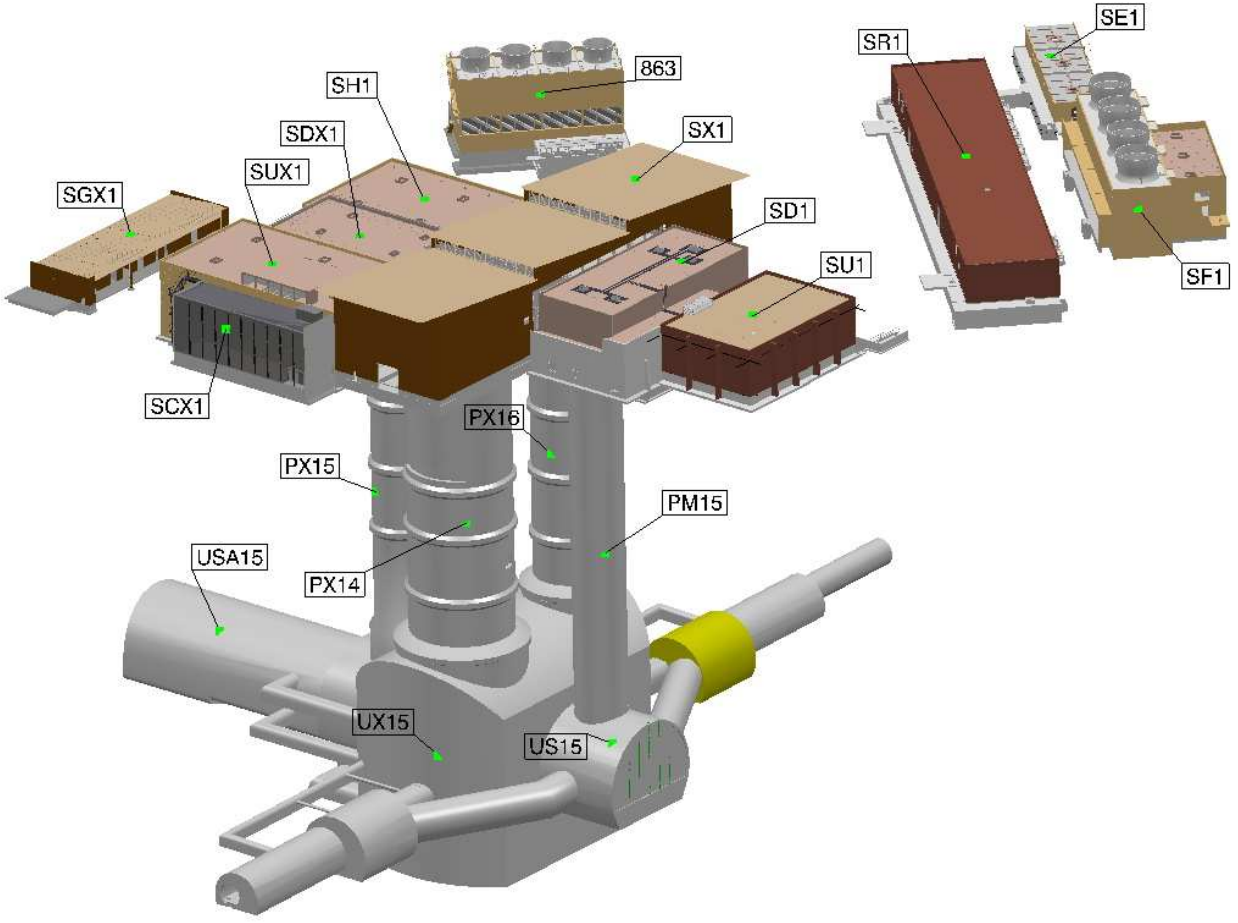
\includegraphics[width=\linewidth,height=\textheight,keepaspectratio]{trigger/facilities}
        \caption{General layout of buildings and facilities at LHC Point 1, site of ATLAS \cite{trigger_tdr}}
        \label{fig:facilities}
    \end{figure}


\section{Level 1 Trigger}
    One bunch-crossing every 25 ns is a blistering pace to operate at.
    The first layer of the trigger system, L1, therefore must run entirely through hardware-level gate logic.
    The goal of this system is to reduce the event rate from the raw 40 MHz bunch-crossing rate, down to a more manageable rate of 100 kHz \cite{trigger_run2}.
    To reduce latency as much as possible, all the electronics comprising L1 are located as close as possible to ATLAS itself, specifically in the USA15 underground chamber \cite{trigger_tdr} (see figure \ref{fig:facilities}).
    As yet another consequence of the high frequency L1 must operate at, it exclusively uses information from the ATLAS calorimeters and Muon Trigger Chamber for its decisions.
    %(utilizes detector buffer memory to keep up).

    The Muon Trigger aspect of L1 is based entirely on the trigger-dedicated Muon Trigger Chamber, described in section \ref{sec:muon-trigger_chamber}.
    Its purpose is to make trigger decisions primarily based on muon $p_T$ and track multiplicity in the Trigger Chamber \cite{trigger_run1}.
    In the calorimeter-based trigger, the selection algorithm first requires a reduction in data resolution.
    The full granularity of the ATLAS calorimeters is too complex to analyze in the 25 ns L1 has to process each bunch-crossing.
    Instead, the various sensors of the calorimeters are clustered together into ``trigger towers", each with a resolution of 0.1x0.1 in $\Delta \eta \times \Delta \phi$.
    The way towers are clustered and used varies between the different L1 calorimeter trigger modules: the CPM, JEM, and CMX.

    \begin{figure}[h]
        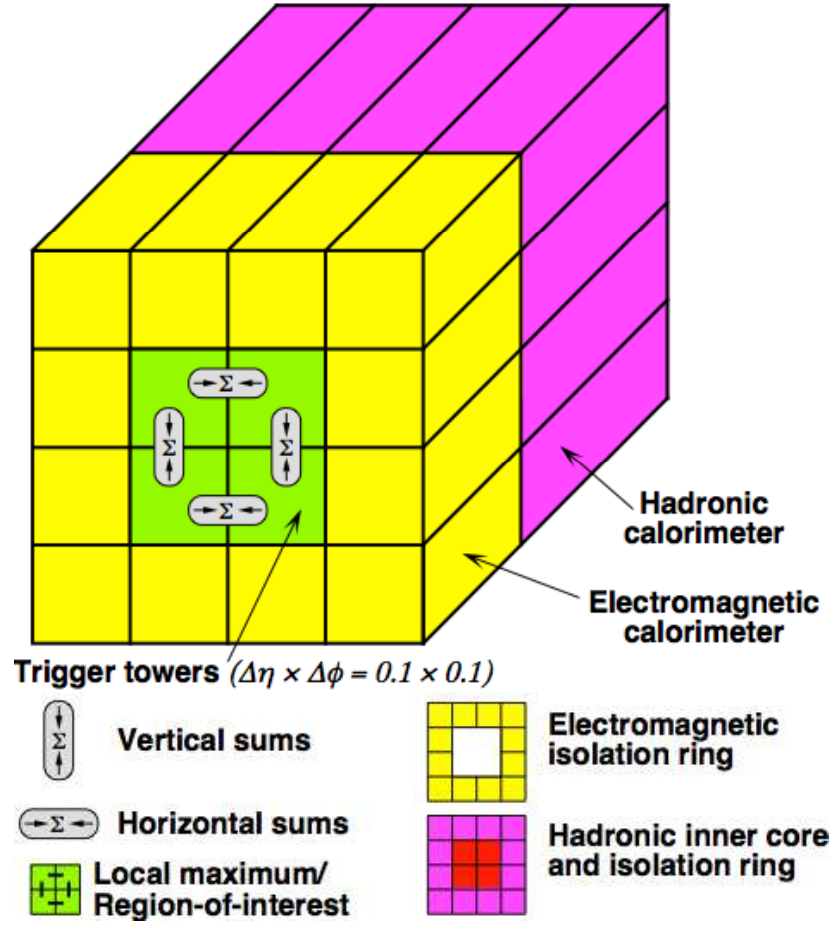
\includegraphics[width=\linewidth,height=\textheight,keepaspectratio]{trigger/trigger_towers}
        \caption{Structure of trigger towers and Regions of Interest \cite{L1_calo_run1}}
        \label{fig:trigger_towers}
    \end{figure}


    The Cluster Processor Module (CPM) exclusively uses the Barrel Calorimeters to function, and is primarily meant for rapid identification of electrons/photons and taus/hadrons.
    For either case, the CPM's first step is to check all possible 4x4 ``windows" of trigger towers, identifying windows containing an isolated ``Region of Interest" (RoI).
    Here, an RoI is defined as a 2x2 cluster of towers with an $E_T$ sum that is a relative maximum compared to surrounding towers.
    This 2x2 RoI is the center of the 4x4 window (see figure \ref{fig:trigger_towers}).
    Windows are considered as passing the CPM trigger if the RoI satisfies an isolation requirement, meaning that the 12 towers surrounding that core fall \textit{below} a predefined $E_T$ ``isolation threshold" value.
    Electrons and photons are then separated from taus and hadrons by the fact that the latter group penetrates into the HCal barrel, while the former group stays highly contained to the ECal.

    Expanding out, the Jet/Energy Processing Module (JEM, or sometimes JEP) makes use of the calorimeter barrels and endcaps, as well as the FCAL, though it does not distinguish between the ECal and HCal.
    The JEM further reduces the granularity under consideration, with a basic unit of data collection being 2x2 collections of trigger towers called ``jet elements", resulting in a minimum resolution of 0.2x0.2 in $\Delta \eta \times \Delta \phi$.
    Like the CPM, the JEM runs its trigger conditions on windows of multiple jet elements that must be based around a 2x2 RoI core (which is a local $E_T$ maximum).
    Unlike the CPM, these windows can vary in size.
    Primarily, the JEM is intended to perform hit multiplicity counting as well as assist the Extended Cluster Merger Modules (CMX) in carrying out the final jet multiplicity and $E_T$ sums \cite{L1_calo_run1}\cite{trigger_run2}.
    When these conditions, alongside those performed in the Muon trigger, are completed, the event is passed along to the HLT.


\section{High Level Trigger}
    After the L1 Trigger has reduced the event rate to 100 kHz, the software-based High Level Trigger is used to further reduce the event rate to the final output of \textasciitilde 1 kHz.
    Located in the SCX1 building (figure \ref{fig:facilities}) at the surface of P1 (again to minimize latency), the HLT uses data from all detector elements to completely reconstruct the event as it occurred in ATLAS, and performs its selections based on this reconstructed event.
    Different physics processes and particles, known as physics ``signatures", are reconstructed in different ways, and have different triggers based around them. 
    The main signatures used in ATLAS are: minimum bias signatures, electron/photons (Egamma), muons, jets, taus, missing transverse energy (MET), b-jets (as in jets from bottom quarks), and B-physics (as in B-hadrons).
    The process of reconstruction and the trigger algorithms applied to these reconstructed signatures are based on offline software algorithms which have been repurposed for online use.
    These offline algorithms are quite technical in nature, and are discussed further in chapter [TODO].
    However, once events have successfully passed both L1 and the HLT, they are finally distributed off-site for analysis by different physics groups.


\section{Scale Factors} %TODO
    We use these pretty extensively in 4b with the weird online-tagged/offline-tagged event weighting system.
    So I do unfortunately need to revisit this.
